\graphicspath{{4sets/asy/}}
\section{Sets and Functions}\label{chap:sets}


Sets are the fundamental building blocks of mathematics, providing the language necessary for describing mathematical objects and for grouping objects together according to shared characteristics. Understanding how to read and effectively employ set notation is our primary focus. The mathematical discipline of \emph{set theory} is, however, far more ambitious than this. Set theorists define all basic mathematical objects---\emph{numbers, addition, functions,} etc.---purely in terms of sets, an impractical approach for most working mathematicians, most of the time.\footnote{Within \emph{axiomatic set theory} it can take over 100 pages to justify writing $1+1=2$. The difficulty is that rigorous definitions---using sets---are first required of the notions \emph{one, two, equals} and \emph{add}\ldots} We will only scratch the surface of this. Indeed long before one can accept that such an approach has its place in mathematics, a significant level of familiarity with sets and their basic operations is necessary.


\subsection{Set Notation and Subsets}\label{sec:subset}

Without any attempt to define the meaning of \emph{object,} we start with a naïve definition.

\begin{defn}[lower separated=false, sidebyside, sidebyside align=top seam, sidebyside gap=0pt, righthand width=0.3\linewidth]{}{}
	A \emph{set} is a collection of objects, its \emph{elements} or \emph{members.}\smallbreak
	The notation $x\in A$ is read ``$x$ is an \emph{element}/\emph{member} of the set $A$,'' or more often simply ``$x$ is in $A$.'' Otherwise said, $x$ is an object in the collection labelled $A$.\smallbreak
	If $y$ is a member of some other set, but not of $A$, we write $y\notin A$ (``$y$ is not in $A$'').\smallbreak
	\tcblower
	\flushright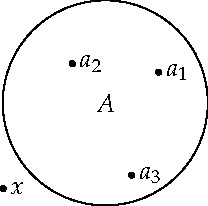
\includegraphics{sets-01-venn}
\end{defn}

As in the definition, it is typical to use upper-case letters ($A,B,C,\ldots$) for abstract sets and lower-case letters for their elements.\smallbreak

\emph{Venn diagrams} are useful for visualizing abstract sets. A set is represented by a region in the plane, with elements depicted by dots. The diagram in the definition represents a set $A$ comprising at least four elements $a_1,a_2,a_3$ and $x$. The element $y$ does not lie in $A$. 

\begin{example}{}{}
	Let $A$ be the set of (names of) US states. Then Michigan $\in A$ and Saskatchewan $\notin A$.
\end{example}

\begin{defn}{}{subset}
	Let $A$ and $B$ be sets.
	\begin{enumerate}
	  \item Sets are \emph{equal,} written $A=B$, if they have precisely the same elements.\par
	  \begin{minipage}[t]{0.74\linewidth}\vspace{-4pt}
	  	\item $A$ is a \emph{subset} of $B$, written $A\subseteq B$, if every element of $A$ is also an element of $B$.
	  	\item $A$ is a \emph{proper subset} of $B$ if $A\subseteq B$ and $A\neq B$. To stress this, we'd write $A\subsetneq B$. The Venn diagram on the right represents a proper subset. 
	  \end{minipage}
	  \hfill
	  \begin{minipage}[t]{0.25\linewidth}\vspace{-15pt}
			\flushright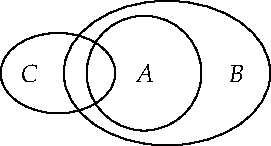
\includegraphics{sets-02-vennsubset}
	  \end{minipage}
	\end{enumerate}
\end{defn}

The following observations are simply translations of the definition:
\begin{enumerate}
  \item Equality: $A=B \iff A\subseteq B$ and $B\subseteq A$.
  \item Subset: $A\subseteq B \iff \bigl(x\in A\Longrightarrow x\in B\bigr) \iff \bigl(\forall x\in A, x\in B\bigr)$
  \item Not a subset: $A\nsubseteq B \iff \exists x\in A$ for which $x\notin B$.
\end{enumerate}


\boldsubsubsection{Roster \& Set-Builder Notation}

\emph{Roster notation} is the most basic way to describe the elements of a set: simply \emph{list} the elements in any order between curly brackets $\{\,,\,\}$.

\begin{example}{}{easysetnotation}
	Let $A$ be the set of (real number) solutions to the equation $2x^2-7x+3=0$ and let $B$ be the set of \emph{integer} solutions to the same equation. Since the polynomial factorizes as $(2x-1)(x-3)$, we see that $A=\{3,\frac 12\}$ and $B=\{3\}$. We could also write $A=\{\frac 12,3\}$ since \emph{order doesn't matter in roster notation.}	Moreover:
	\begin{itemize}
	  \item $A\nsubseteq B$ since $\frac 12\in A$ and $\frac 12\notin B$.
	  \item $B\subseteq A$ since 3 (the only element of $B$) lies in $A$. Indeed $B\subsetneq A$ is a  proper subset since $A\neq B$.
	\end{itemize}
\end{example}

Roster notation is ideal for small sets, but is of limited utility when trying to describe large sets. This is where our second notation rides to the rescue.\bigbreak

\emph{Set-builder notation} describes the elements of a set using some common property. Suppose $\cU$ is some (already understood) set and $P(x)$ is a propositional function with domain $\cU$, then
\[
	A:=\bigl\{x\in\cU:P(x)\bigr\} \tag{``$A$ is the set of $x$ in $\cU$ such that $P(x)$''}
\]
defines a set $A$ as \emph{the subset} of $\cU$ all of whose elements $x$ satisfy the property $P(x)$. A vertical separator $\mid$ is often used instead of a colon: we'll use both, though it might be essential in a given context to use one rather than the other for clarity.

\begin{examples}{}{}
\exstart Continuing Example \ref{ex:easysetnotation}, recall that $\R$ represents the set of real numbers and $\Z$ the set of integers. In set-builder notation, our solution sets may be written
	\[A=\bigl\{x\in\R:2x^2-7x+3=0\bigr\},\qquad B=\bigl\{x\in\Z:2x^2-7x+3=0\bigr\}\]
	In this case the qualifying proposition $P(x)$ is ``$2x^2-7x+3=0$.''
	\begin{enumerate}\setcounter{enumi}{1}
	  \item[]We can also express the fact that $B$ is a subset of $A$ in this notation (this time with a vertical separator),
	\[B=\bigl\{x\in A\bigm| x\in\Z\} \tag{``the set of elements $x$ in $A$ such that $x$ is an integer"}\]
	
	\item Let $X=\{2,4,6\}$ and $Y=\{1,2,5,6\}$. There are many options for how to write these in set-builder notation. For instance:
	\[
		X=\bigl\{n\in\Z:\tfrac 12n\in\{1,2,3\}\bigr\},\qquad Y=\bigl\{n\in\Z\bigm|1\le n\le 6\text{ and }n\neq 3,4\bigr\}
	\]
	We now practice the opposite skill by converting five sets from set-builder to roster notation.
	\begin{align*}
		&S_1=\bigl\{x\in X:x\text{ is divisible by 4}\bigr\}=\{4\}
		&&
		S_2=\bigl\{y\in Y:y\text{ is odd}\bigr\}=\{1,5\}
		\\
		&S_3=\bigl\{x\in X\bigm| x\in Y\bigr\}=\{2,6\}
		&&
		S_4=\bigl\{x\in X:x\notin Y\bigr\}=\{4\}
		\\
		&S_5=\bigl\{y\in Y\bigm| y\text{ is odd and $y-1\in X$}\}=\{5\}
	\end{align*}
	Can you find alternative descriptions in set-builder notation for the sets $S_1,\ldots,S_5$ above? Take your time getting used to this notation: the ability to translate between various descriptions of a set is \emph{crucial} to reading mathematics!
	
	\item We use the set $C=\{0,1,2,3,\ldots,24\}$ to describe $D=\{n\in\Z:n^2-3\in C\}$ in roster notation. Start by expanding the criterion for membership in $D$:
  \[
  	n^2-3\in C\iff n^2\in\bigl\{3,4,5,\ldots,25,26,27\bigr\}
  \]
  Since $n$ must be an integer, it follows that $D=\{\pm 2,\pm 3,\pm 4,\pm 5\}$.
  
  \item To express $E=\{0,2,6,12,\ldots\}$ in set-builder notation we might spot a pattern and decide that
  \[
  	E=\bigl\{n\in\Z: n=m(m+1) \text{ for some integer }m\ge 0\bigr\}
  \]
  The problem is that we cannot guarantee our correctness! Perhaps the correct formula is
  \[
  	n=m(m+1)+m(m-2)(m-6)(m-12)
  \]
	In the first case the next term in the sequence is $4\cdot 5=20$, whereas in the second case it is $20+128=148$. For larger sets, the clarity afforded by set-builder notation is essential!

	\end{enumerate}
\end{examples}



\boldsubsubsection{Common Sets of Numbers}

We've used some of this notation already, and much of the rest should be familiar.\vspace{-5pt}

\begin{quote}\def\arraystretch{1.15}
	\begin{tabular}{@{}ll}
		\emph{Natural numbers}&$\N=\bigl\{1,2,3,4,\ldots\bigr\}$ is the set of \emph{positive} integers.\\
		\emph{Integers}&$\Z=\bigl\{\ldots,-3,-2,-1,0,1,2,3,\ldots\bigr\}$.\\
		\emph{Rational numbers}&$\Q=\bigl\{\frac mn:m\in\Z\text{ and }n\in\N\bigr\} =\bigl\{\frac ab\bigm| a,b\in\Z\text{ and }b\neq 0\bigr\}$.\\
		\emph{Real numbers}&$\R$. Even a rudimentary definition is too involved for this text.\footnotemark\\
		\emph{Complex numbers}&$\C=\bigl\{x+iy:x,y\in\R\bigr\}$ where $i^2=-1$. We won't use these.
	\end{tabular}
\end{quote}

\vspace{-10pt}
	
\footnotetext{We simply assume the reader is comfortable with the idea of the real line where number corresponds to \emph{length.} A rigorous development of $\R$ is a matter for an upper-division \emph{analysis} course.}

\begin{examples}{}{}
	\exstart For instance: \ $7\in\N$, \ $\pi\in\R$, \ $-\frac 79\notin\Z$, \ $\sqrt 2\notin\Q$ \ and \ $3+\sqrt 5i\in\C$.
	\begin{enumerate}\setcounter{enumi}{1}%\itemsep2pt
	  \item The basic symbols can be decorated to make natural modifications. For example:
\vspace{-3pt}
		\begin{itemize}
		  \item $\N_0=\bigl\{0,1,2,3,4,\ldots\bigr\}=\Z^+_0=\bigl\{x\in\Z:x\ge 0\bigr\}$. Also called the \emph{whole numbers} ($\mathbb W$).
			\item $\Z_{\ge 5}=\bigl\{5,6,7,8,\ldots\bigr\} =\bigl\{x\in\Z:x\ge 5\bigr\}$ denotes the integers greater than or equal to 5.
		  \item $\R^+=\bigl\{x\in\R:x>0\bigr\}$ is the set of positive real numbers.
			\item $4\Z=\bigl\{\ldots,-8,-4,0,4,8,12,\ldots\bigr\} =\bigl\{x\in\Z: 4\mid x\bigr\}$ is the set\footnotemark{} of integer multiples of 4.\par
			This notation can be used for non-integer multiples, e.g. $\pi\Z=\bigl\{\ldots,-\pi,0,\pi,2\pi,\ldots\bigr\}$. 
			\item $2\Z+1=\bigl\{x\in\Z:x\equiv 1\pmod 2\bigr\}$ is the set of odd integers.
		\end{itemize}
		
		\item \emph{Intervals} are the most commonly encountered subsets of the real numbers. For instance:
% \vspace{-3pt}
		\begin{itemize}
		  \item $[1,\pi]=\bigl\{x\in\R\bigm|1\le x\le \pi\bigr\}$ is a \emph{closed} interval 
		  \item $[-4,7.21)=\{x\in\R\bigm|-4\le x<7.21\}$ is a \emph{half-open} interval.
		  \item $(-\infty, \sqrt 2) =\{x\in\R\bigm|x<\sqrt 2\}$ is an \emph{infinite (open)} interval.
		\end{itemize}
	\end{enumerate}
\end{examples}

\vspace{-5pt}

\footnotetext{Be careful!---the colon is the ``such that" separator while $\mid$ denotes the property ``4 divides $x$.''} %The unreadability of $\bigl\{x\in\Z\bigm| 4\mid x\bigr\}$ illustrates the benefit of having two separator symbols to choose from.}

\goodbreak

In view of the natural subset relationships $\N\subsetneq\Z\subsetneq\Q\subsetneq\R\subsetneq\C$, we consider a simple result.

\begin{lemm}{Transitivity of Subset}{subsettrans}
	Suppose $A\subseteq B$ and $B\subseteq C$. Then $A\subseteq C$.
\end{lemm}

\begin{proof}
	Think back to the criteria following Definition \ref{defn:subset}. Suppose $A\subseteq B$ and $B\subseteq C$. Then
	\[
		x\in A \overset{(A\subseteq B)}{\implies} x\in B\overset{(B\subseteq C)}{\implies} x\in C
	\]
	We conclude that $A\subseteq C$.
\end{proof}

Compare this to Exercise \ref*{sec:prop}.\ref{exs:iftransitive}: if we translate each subset relation into an implication, the proof structure is $(x\in A\Rightarrow x\in B)\wedge (x\in B\Rightarrow x\in C)\Longrightarrow (x\in A\Rightarrow x\in C)$. This is typical of basic results about sets: after translation, the theorem reduces to one of the standard rules of logic.



\boldsubsubsection{Cardinality and the Empty Set}

It is helpful to introduce some terminology to describe the \emph{size} of a set.

\begin{defn}{}{}
	A \emph{finite set} contains only a finite number of elements: this number is its \emph{cardinality,} written $\nm A$. A set with infinitely many elements is said to be an \emph{infinite set.}\par
	The symbol $\emptyset$ denotes the \emph{empty set}: a set containing no elements (cardinality zero: $\nm\emptyset=0$).
\end{defn}



\begin{examples}{}{}
	\exstart Let $A=\bigl\{1,3,\pi,\sqrt 2,103\bigr\}$, then $\nm A=5$.
	\begin{enumerate}\setcounter{enumi}{1}
		\item Let $B=\bigl\{4,\{1,2\},\{3\}\bigr\}$. The elements of $B$ are $4$, $\{1,2\}$ and $\{3\}$, therefore $\nm B=3$. It doesn't matter that the \emph{element} $\{1,2\}\in B$ is also a set!\par
		\begin{minipage}[t]{0.59\linewidth}\vspace{-5pt}
			\item Recall some basic trigonometry:
			\[
				\left\{x\in[0,4\pi]:\cos x=\frac 12\right\}=\left\{\frac{\pi}3,\frac{5\pi}3,\frac{7\pi}3,\frac{11\pi}3\right\}
			\]
			has cardinality 4.
		\end{minipage}
		\hfill
		\begin{minipage}[t]{0.4\linewidth}\vspace{-10pt}
			\flushright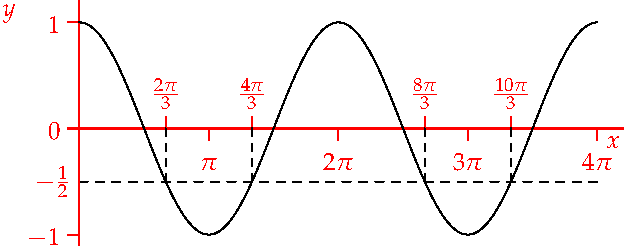
\includegraphics{sets-03-cos}
		\end{minipage}
		
		\item There are many representations of the empty set: for example
		\[
			\emptyset =\bigl\{x\in\R:x^2=-1\bigr\} = \bigl\{x\in\N:x^2+3x+2=0\bigr\}=\bigl\{n\in\N:n<0\bigr\}
		\]
		In general, if $X$ is any set and $P(x)$ is false for all $x\in X$, then\footnotemark{} $\emptyset=\bigl\{x\in X:P(x)\bigr\}$.
	\end{enumerate}
\end{examples}

\footnotetext{In some formalizations of set theory, the existence of the empty set is an axiom: an assumption made without proof. Provided one accepts that set-builder notation always defines a set---this is itself an axiom!---and that at least one set $X$ exists, the empty set may be \emph{defined} as in the example: a suitable property $P(x)$ might be something like ``$x\notin\{x\}$.''}


Cardinality is a very simple concept for finite sets; if $B$ is finite, so is any subset, and we have
\[
	A\subseteq B\implies \nm A\le \nm B
\]
For infinite sets, cardinality is more subtle. We'll return to this issue and uncover some of the bizarre and fun consequences of infinite cardinalities in Chapter \ref{chap:cantor}.
\bigbreak

We finish with a couple of simple results regarding the empty set.

\begin{lemm}{}{emptysetunique}
	Let $A$ be a set.
	\begin{enumerate}
	  \item If $\nm A=0$, then $A=\emptyset$. The empty set is \emph{the unique set} with zero cardinality.
	  \item $\emptyset\subseteq A$ and $A\subseteq A$
	\end{enumerate}
\end{lemm}

\begin{proof}
	Think about the claim $\emptyset\subseteq A$: by the observations following Definition \ref{defn:subset}, this means
	\[
		x\in\emptyset\implies x\in A
	\]
	This is true (for any set $A$!) since there are no elements $x$ satisfying the hypothesis.\footnotemark{}
	\begin{enumerate}
 	 \item Suppose $A$ has cardinality zero. Repeating and combining with the above observation, we see that $\emptyset\subseteq A$ and $A\subseteq\emptyset$. We conclude that $A=\emptyset$.
 	 \item We already know that $\emptyset\subseteq A$. For the second part, simply observe that
 	 $x\in A\implies x\in A$.\qedhere
\end{enumerate}
\end{proof}

\footnotetext{If $P(x)$ is always false, then $(\forall x)\ P(x)\Longrightarrow Q(x)$ is true. This is called a \emph{vacuous} (empty) theorem.}

% 
% 
% \begin{examples}{}{}
% 	\begin{enumerate}\setcounter{enumi}{1}
%   \item Are the following sets equal?
%   \[E=\{n^2+2\in\Z:\text{$n$ is an odd integer}\},\qquad F=\{n\in\Z:n^2+2\text{ is an odd integer}\}.\]
%   It may help to first construct a table listing some of the values of $n^2+2$:
%   \[\begin{array}{c|c|c}
%   n&n^2&n^2+2\\\hline
%   \pm 1&1&3\\
%   \pm 3&9&11\\
%   \pm 5&25&27\\
%   \pm 7&49&51\\
%   \pm 9&81&83\\[-5pt]
%   \vdots&\vdots&\vdots
%   \end{array}\]
%   The set $E$ consists of those integers of the form $n^2+2$ where $n$ is an odd integer. By the table,
%   \[E=\{3,11,27,51,83,\ldots\}.\]
%   On the other hand, $F$ includes all those integers $n$ such that $n^2+2$ is odd. It is easy to see that
%   \[n^2+2\text{ is odd}\iff n^2\text{ is odd}\iff n\text{ is odd.}\]
%   Thus $F$ is simply the set of all odd integers:
%   \[F=\{\pm 1,\pm 3,\pm 5,\pm 7,\ldots\}=2\Z+1.\]
%   Plainly the two sets are not equal.
% 
%   \item $\{x\in\R:x^2-1=0\}\subseteq \{y\in\R:y^2\in\N\}$.\\
%   To make sense of this relationship, convert to roster notation: we obtain
%   \[\{-1,1\}\subseteq\{\pm\sqrt 1,\pm\sqrt 2,\pm\sqrt 3,\pm\sqrt 4,\ldots\}.\]
%   \item If $m$ and $n$ are positive integers, then $m\Z\subseteq n\Z\iff n\mid m$. Make sure you're comfortable with this! For example, $4\Z\subseteq 2\Z$ since every multiple of 4 is also a multiple of 2.
% \end{enumerate}
% \end{examples}


% \paragraph{Self-test Questions}
% 
% \begin{enumerate}
%   \item True or false: An open interval contains its endpoints.
%   \item True or false: $\{x\in\R:x^2<0\}$ is a representation of the empty set.
%   \item True or false: $\{x\in\Z:x\in[0,4)\}=\{0,1,2,3,4\}$.
% \end{enumerate}


\begin{exercises}{}{}
	A reading quiz and several questions with linked video solutions can be found \href{http://www.math.uci.edu/~ndonalds/math13/selftest/4-1-subset.html}{online}.


% Write the set $A=\{x\in\R:x^2+3x+2=0\}$ in roster notation.\\[5pt]
% 	We are looking for the set of all real number solutions to the quadratic equation $x^2+3x+2=0$. A simple factorization tells us that $x^2+3x+2=(x+1)(x+2)$, whence $A=\{-1,-2\}$.

	\begin{enumerate}
	  \item Describe the following sets in roster notation: that is, list their elements.
		\begin{enumerate}
		  \item \makebox[215pt][l]{$\bigl\{x\in\N:x^2\le 3x\bigr\}$\hfill (b)} \ $\bigl\{n\in\{0,1,2,3,\ldots,19\}:n+3\equiv 5\spmod 4\bigr\}$
		  \setcounter{enumii}{2}
		  \item \makebox[215pt][l]{$\bigl\{n\in\{-2,-1,0,1,\ldots,23\}:4\mid n^2\bigr\}$\hfill (d)} \ $\bigl\{x\in \frac 12\Z: 0\le x\le 4\text{ and }4x^2\in 2\Z+1\bigr\}$
		  \setcounter{enumii}{4}
		  \item $\bigl\{y\in\R:y=x^2\text{ for some $x\in\R$ with } x^2-3x+2=0\bigr\}$
		\end{enumerate}
			
			
		\item Describe the following sets in set-builder notation (\emph{look for a pattern}).
		\begin{enumerate}
		  \item \makebox[180pt][l]{$\bigl\{\ldots,-3,0,3,6,9,\ldots\bigr\}$\hfill (b)} \ $\bigl\{-3,1,5,9,13,\ldots\bigr\}$
		  \setcounter{enumii}{2}
		  \item $\bigl\{1,\frac 13,\frac 17,\frac 1{15},\frac 1{31},\ldots\bigr\}$
		\end{enumerate}
		  
	
	  \item Each of the following sets of real numbers is a single interval. Determine the interval.
		\begin{enumerate}
		  \item \makebox[180pt][l]{$\bigl\{x\in\R:x>3\text{ and }x\le 17\bigr\}$\hfill (b)} \ $\bigl\{x\in\R:x\nleq 3\text{ or }x\le 17\bigr\}$
		  \setcounter{enumii}{2}
		  \item \makebox[180pt][l]{$\bigl\{x^2\in\R:x\neq 0\bigr\}$ \hfill (d)} \ $\bigl\{x\in\R^-:x^2\ge 16\text{ and }x^3\le 27\bigr\}$
		\end{enumerate}
			
			
		\item Is the set $\{x\in\Z:-1\le x<43\}$ finite or infinite? If finite, what is its cardinality?
				
		
		%\item Compare the sets $A=\{3x\in\Z:x\in 2\Z\}$ and $B=\{x\in\Z:x\equiv 12\pmod 6\}$. Are they equal?
			
			
		\item What is the cardinality of the set $\Bigl\{\emptyset,\bigl\{\emptyset\bigr\},\bigl\{\emptyset,\{\emptyset\}\bigr\}\Bigr\}$? \ What are its elements?
		
		\item Let $A=\emptyset$, \ $B=\{A\}$, \ $C=\bigl\{\{A\}\bigr\}$ \ and \ $D=\bigl\{A,\{0\},\{0,1\}\bigr\}$.\par
	  Answer the following true or false:
	  \begin{enumerate}
	    \item \makebox[80pt][l]{$0\in A$\hfill (b)} \ \makebox[80pt][l]{$A\in B$\hfill (c)} \ \makebox[80pt][l]{$A\in C$\hfill (d)} \ \makebox[80pt][l]{$B\in C$ \hfill (e)} \ $A\in D$
	    \setcounter{enumii}{5}
	    \item \makebox[80pt][l]{$B\in D$\hfill (g)} \ \makebox[80pt][l]{$0\in D$\hfill (h)} \ \makebox[80pt][l]{$\{0\}\in D$\hfill (i)} \ $\{1\}\in D$
	  \end{enumerate}
	  
	  
	  \item List all the \emph{proper} subsets of $\{1,2,3\}$.
	  
	    
		\goodbreak
	   
		   
		\item Let $A,B,C,D$ be the following sets:
	  \begin{align*}
	  	&A=\{-4,1,2,4,10\}
	  	&&B=\bigl\{m\in\Z:\nm m\le 12\bigr\}\quad \text{(\emph{absolute value of $m$})}\\
	  	&C=\bigl\{n\in\Z:n^2\equiv 1\spmod 3\bigr\}
	  	&&D=\bigl\{t\in\Z:t^2+3\in [4,20)\bigr\}  
	  \end{align*}
	  Of the 12 subset relations $A\subseteq B$,\ $A\subseteq C,\ldots, D\subseteq C$, which are true and which false?
	  
	  \item Let $A=\bigl\{1,2,\{1,2\},\{3\}\bigr\}$ and $B=\{1,2\}$. Answer the following true or false:
	  \begin{enumerate}
	    \item \makebox[100pt][l]{$B\in A$\hfill (b)} \ \makebox[100pt][l]{$B\subseteq A$\hfill (c)} \ \makebox[100pt][l]{$3\in A$\hfill (d)} \ $\{3\}\subseteq A$
	    \setcounter{enumii}{4}
	    \item \makebox[100pt][l]{$\{3\}\in A$\hfill (f)} \ \makebox[100pt][l]{$\emptyset\subseteq A$\hfill (g)} \ $\emptyset\in A$
	  \end{enumerate}
	  
	  \item Let $A=\{0,2,4,6,8,10\}$. Write the set $B=\{X\subseteq A:|X|=2\}$ in roster notation.
	  
	    
	  \item\begin{enumerate}
	    \item Suppose $A\subseteq B\subseteq C\subseteq A$. Show that $A=B=C$.
	    \item Is it possible for sets $A,B,C$ to satisfy $A\subsetneq B\subseteq C\subseteq A$? Why/why not?
	  \end{enumerate}

	
		\item Let $A=\{\text{1,2,3,4}\}$, and let $B =\bigl\{\{x,y\}:x,y\in A\bigr\}$.
		\begin{enumerate}
	  	\item Describe $B$ in roster notation (\emph{what happens when $x=y$?}).
			\item Find the cardinalities of the following sets:
			\[
				C=\Bigl\{\bigl\{x,\{y\}\bigr\}:x,y\in A\Bigr\}
				\quad\text{and}\quad
				D=\biggl\{\Bigl\{\bigl\{x,\{y\}\bigr\}:x,y\in A\Bigr\}\biggr\}
			\]
		\end{enumerate}
  
  
  	\item Let $A=\{x\in\R:x^3+x^2-x-1=0\}$ and $B=\{x\in\R:x^4-5x^2+4=0\}$. Are either of the relations $A\subseteq B$ or $B\subseteq A$ true? Explain.
  
  
  	\item For which real numbers $x>0$ do we have $[0,x]\subsetneq[0,x^2]$? Prove your assertion.
  
  
  	\item Let $m,n\in\N$. Prove: $m\Z\subseteq n\Z\iff n\mid n$.

  
  	\item\label{ex:mirrored} Given $A\subseteq\Z$ and $x\in\Z$, we say that $x$ is $A$-mirrored if and only if $-x\in A$. Also define
  	\[
			M_A:=\bigl\{x\in\Z: x\text{ is $A$-mirrored}\bigr\}
		\]
		\begin{enumerate}
	  	\item What does it mean for $x$ \emph{not} to be $A$-mirrored?
	  	\item Find $M_B$ given $B=\{0,1,-6,-7,7,100\}$.
	  	\item Assume that $A \subseteq\Z$ is closed under addition: for all $x,y\in A$, we have $x+y\in A$. Show that $M_A$ is closed under addition.
	  	\item In your own words, under which conditions is $A=M_A$?
		\end{enumerate}

  \item Define the set $[1]=\bigl\{x\in\Z: x\equiv 1\spmod 5\bigr\}$.
		\begin{enumerate}
		  \item Describe the set $[1]$ in roster notation.
		  \item Compute the set $M_{[1]}$, as defined in Exercise \ref{ex:mirrored}. Is $M_{[1]}$ equal to $[1]$?
			\item Now consider the set $[10]=\{x\in\Z:x\equiv 10\spmod 5\}$. Are the sets $[10]$ and $M_{[10]}$ equal? Prove or disprove.
  	\end{enumerate}


     % \item (Hammack's \href{http://www.people.vcu.edu/~rhammack/BookOfProof/}{\emph{Book of Proof}}, Section 1.3, Exercise 6)
%List all subsets of $\{\R,\Q,\N\}$.
    

		\item Consider the set $A=\{a,b,c,d\}$. 
    \begin{enumerate}
      \item Of each cardinality 0, 1, 2, 3 and 4, how many subsets has $A$? Is there a pattern?
        
      \item Completely expand the polynomial $(1 + x)^4$. What do you notice about the coefficients? 
    \end{enumerate}

	\end{enumerate}
\end{exercises}

\clearpage



\subsection{Unions, Intersections and Complements}\label{sec:union}

In this section we construct new sets from old, modeled precisely on the logical concepts of \emph{and, or,} and \emph{not} (compare Definition \ref{defn:andornot}). 


\begin{defn}{}{unionint}
	Let $\cU$ be a (universal) set,\footnotemark{} and suppose $A,B$ are subsets of $\cU$.
	\begin{enumerate}\itemsep0pt
		\item The \emph{union} of $A$ and $B$ is the set of elements in $A$ or $B$:
		\[
			\makebox[210pt][l]{$A\cup B:=\bigl\{x\in\cU:x\in A\text{ or }x\in B\bigr\}$\hfill} (x\in A\cup B\iff x\in A\text{ or }x\in B)
		\]
		\item The \emph{intersection} of $A$ and $B$ is the set of elements in both $A$ and $B$:
		\[
			\makebox[210pt][l]{$A\cap B:=\bigl\{x\in\cU:x\in A\text{ and }x\in B\bigr\}$\hfill} (x\in A\cap B\iff x\in A\text{ and }x\in B)
		\]
		We say that $A$ and $B$ are \emph{disjoint} if $A\cap B=\emptyset$.
	  \item The \emph{complement} of $A$ is the set of all elements not in $A$:
		\[
			\makebox[210pt][l]{$\comp A:=\bigl\{x\in\cU:x\notin A\bigr\}$ \hfill} (x\in\comp A\iff x\notin A \ (\text{and }x\in\cU))
		\]
		This can be read ``$B$ minus $A$'', indeed some authors write $B-A$. Similarly $\comp A=\cU\setminus A$, etc.
		\item The \emph{complement of $A$ relative $B$} is the set of elements in $B$ which are not in $A$:
		\[
			\makebox[210pt][l]{$B\setminus A:=B\cap \comp A=\bigl\{x\in B:x\notin A\bigr\}$\hfill} (x\in B\setminus A\iff x\in B\text{ and } x\notin A)
		\]
	\end{enumerate}
	
	\begin{center}
		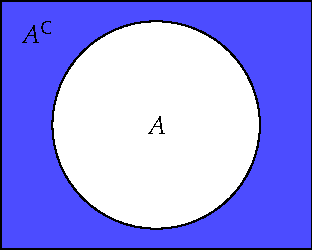
\includegraphics{sets-05-venncomp}
		\qquad\qquad
		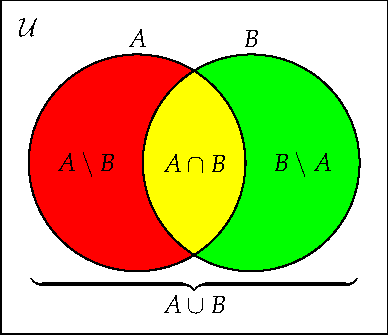
\includegraphics{sets-04-vennunion}
	\end{center}
\end{defn}

\footnotetext{Of which everything else will be a subset. This is needed particularly for complements, but more generally is required to invoke set-builder notation. In certain contexts, the universal set is naturally assumed: $\cU=\R$ makes sense if you are working within the real numbers, $\cU=\Z$ if doing modular arithmetic.}

In the Venn diagrams, the outer box depicts the universal set $\cU$. Though it doesn't constitute a proof, the diagram makes certainly suggests that
\[
	A=(A\setminus B)\cup (A\cap B) \quad\text{and}\quad B=(B\setminus A)\cup(A\cap B)
\]
Observe the notational similarity with logic: $\cup$ looks a bit like $\vee$ (OR); $\cap$ like $\wedge$ (AND).

\begin{examples}{}{}
	\exstart Let $\cU=\{1,2,3,4,5\}$, $A=\{1,2,3\}$, and $B=\{2,3,4\}$. Then
	\begin{align*}
		&\comp A=\{4,5\} &&\comp B=\{1,5\} &&B\setminus A=\{4\} &&A\setminus B=\{1\}\\
		&A\cup B=\{1,2,3,4\} &&A\cap B=\{2,3\} &&A\cap\comp B=\{1\} &&\comp A\cup\comp B=\{1,4,5\}
	\end{align*}
	
	\goodbreak
		
	\begin{enumerate}\setcounter{enumi}{1}
		\item Using interval notation, let $\cU=[-4,5]$, \ $A=[-3,2]$, \ and \ $B=[-4,1)$. Then\par
% 		\begin{align*}
% 			&\comp A=[-4,-3)\cup (2,5] &&\comp B=[1,5] &&A\cup B=[-4,2] \\
% 			&A\setminus B=[1,2] &&B\setminus A=[-4,-3) &&A\cap B=[-3,1) 
% 		\end{align*}
% 		\vspace{-24pt}
% 		\begin{center}
% 		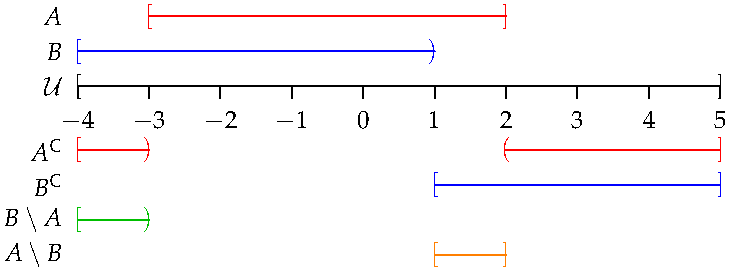
\includegraphics[width=0.7\textwidth]{sets-13-intervalex}
% 		\end{center}
% 		\vspace{-13pt}
		\begin{minipage}[t]{0.3\linewidth}\vspace{-13pt}
			\begin{gather*}
			\comp A=[-4,-3)\cup (2,5]\\
			\comp B=[1,5]\\
			A\setminus B=[1,2]\\
			B\setminus A=[-4,-3)\\
			A\cup B=[-4,2]\\
			A\cap B=[-3,1) 
			\end{gather*}
		\end{minipage}
		\hfill
		\begin{minipage}[t]{0.69\linewidth}\vspace{0pt}
			\flushright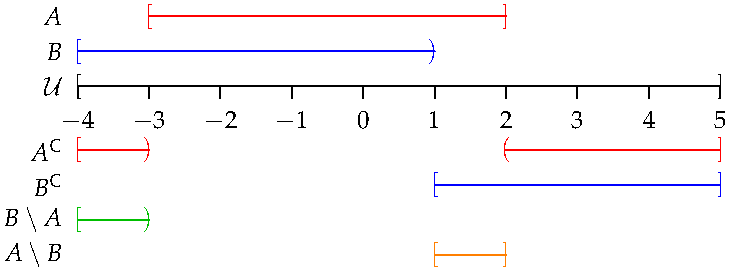
\includegraphics[scale=0.8]{sets-13-intervalex}
		\end{minipage}
		\smallbreak
		While you should be comfortable with these just from the picture, for practice it is worth trying algebraic arguments. In particular, note how $\comp A$ relies on de Morgan's law (Theorem \ref{thm:demorgan}):
		\begin{align*}
			x\in \comp A&\iff x\notin A\iff \neg\bigl(x\in A\bigr) \iff\neg\bigl(-3\le x \text{ and }x\le 2\bigr)\\
			&\iff x<-3\text{ or }x>2 \tag{de Morgan}\\
			&\iff x\in[-4,-3)\cup (2,5] \tag{remember that $x\in\cU$ always!}
		\end{align*}
		
		\item Let $A=(-\infty,3)$ and $B=[-2,\infty)$ in interval notation. Then $A\cup B=\R$ and $A\cap B=[-2,3)$.
	\end{enumerate}
\end{examples}


For the remainder of this section, we summarize the basic rules of set algebra.

\begin{thm}{Union/intersection rules}{setbasic}
	Let $A,B,C$ be sets. Then:
	\begin{enumerate}\itemsep2pt
		\item $\emptyset\cup A=A$ \ and \ $\emptyset\cap A=\emptyset$
		\item $A\cap B\subseteq A\subseteq A\cup B$
		\item $A\cup B=B\cup A$ \ and \ $A\cap B=B\cap A$
		\item $A\cup (B\cup C)=(A\cup B)\cup C$ \ and \ $A\cap (B\cap C)=(A\cap B)\cap C$
		\item $A\cup A=A\cap A=A$
		\item $A\subseteq B\Longrightarrow A\cup C\subseteq B\cup C$ \ and \ $A\cap C\subseteq B\cap C$
	\end{enumerate}
\end{thm}

If you don't believe a result, try \emph{visualizing} it using a Venn diagram. The basic proof strategy is the same for all parts: convert each statement into propositions (Definition \ref{defn:unionint} parentheses) and use what you know from basic logic (e.g., Theorem \ref{thm:demorgan} and page \pageref{pg:asidelogicalgebra}). We prove part 2 and half of part 6, leaving some of the rest to the Exercises.

\begin{proof}
\begin{enumerate}
  \item[2.] There are two results here: $A\cap B\subseteq A$ and $A\subseteq A\cup B$. We prove separately, with some commentary on the side.
	\begin{enumeratea}
		\item Suppose $x\in A\cap B$.\hfill(Goal: want to prove $x\in A\cap B\Rightarrow x\in A$)\par
		Then $x\in A$ and $x\in B$.\hfill(Definition of intersection)\par
		Plainly $x\in A$. We conclude that $A\cap B\subseteq A$\hfill(Definition of subset)
		\item Suppose $y\in A$.\hfill(Goal: prove $y\in A\Rightarrow y\in A\cup B$)\par
		Then ``$y\in A$ or $y\in B$'' is true, whence $y\in A\cup B$.\hfill(Definition of union/or)\par
	  We conclude that $A\subseteq A\cup B$.
	\end{enumeratea}
	
	\goodbreak
	
	\item[6.] (first half)\lstsp Suppose $A\subseteq B$. We wish to prove that $x\in A\cup B\Longrightarrow x\in A\cup C$. However,
	\begin{align*}
		x\in A\cup C&\implies x\in A\text{ or }x\in C\tag{definition of union}\\
		&\implies x\in B\text{ or }x\in C\tag{since $A\subseteq B$}\\
		&\implies x\in B\cup C \tag*{\qedhere}
	\end{align*}
\end{enumerate}
\end{proof}



The next batch of rules describe how complements interact with other set operations: parts 1 and 2 are \emph{de Morgan's laws for sets}; unsurprisingly, their proofs depend on the corresponding laws of logic.


\begin{thm}[lower separated=false, sidebyside, sidebyside align=top seam, sidebyside gap=0pt, righthand width=0.4\linewidth]{Complement rules}{setcomp}
	Let $A,B$ be sets. Then:
	\begin{enumerate}\itemsep2pt
		\item $\comp{(A\cap B)}=\textcolor{blue}{\comp A}\cup \textcolor{red}{\comp B}$ (see picture)
		\item $\comp{(A\cup B)}=\comp A\cap \comp B$
		\item $\smash[t]{\comp{(\comp A)}}=A$
		%\item $A\setminus B=A\cap\comp B$
		\item $A\subseteq B\iff \comp B\subseteq \comp A$
	\end{enumerate}
	\tcblower
	\flushright
	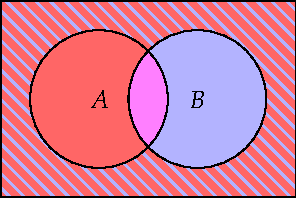
\includegraphics[scale=1]{sets-08-venndemorgan2}
\end{thm}

% \begin{proof}[Proof of 1.]
% We start by trying to show that the left hand side is a subset of the right hand side.
% \begin{align*}
% x\in\comp{(A\cap B)}&\implies x\notin A\cap B\\
% &\implies x\text{ is not a member of \emph{both} $A$ and $B$}\\
% &\implies x\text{ is not in \emph{at least one} of $A$ and $B$}\\
% &\implies x\notin A\text{ or }x\notin B\\
% &\implies x\in\comp A\text{ or }x\in\comp B\\
% &\implies x\in\comp A\cup\comp B
% \end{align*}
% With a little thinking, we realize that all of the $\Longrightarrow$ arrows may be replaced with if and only if arrows $\Longleftrightarrow$ without compromising the argument. We've therefore shown that the sets $\comp{(A\cap B)}$ and $\comp A\cup \comp B$ have the same elements, and are thus equal.
% \end{proof}


\begin{proof}
	We prove only part 1. As before, the natural approach is to restate the result using propositions.
	\begin{align*}
		x\in\comp{(A\cap B)}&\iff \neg\bigl(x\in A\cap B\bigr) \iff \neg\bigl(x\in A\ \text{ and }\  x\in B\bigr)\\
		&\iff \neg\bigl(x\in A\bigr)\ \text{ or }\ \neg\bigl(x\in B\bigr) \tag*{(de Morgan's first law of logic)}\\
		&\iff x\in\comp A\ \text{ or }\ x\in\comp B\\
		&\iff x\in\comp A\cup\comp B\tag*{\qedhere}
	\end{align*}
\end{proof}

Our final pair of results describe the interaction of unions and intersections.\par

\begin{thm}[lower separated=false, sidebyside, sidebyside align=top seam, sidebyside gap=0pt, righthand width=0.3\linewidth]{Distributive laws}{setdist}
	For any sets $A,B,C$:
	\begin{enumerate}\setlength{\itemsep}{2pt}
		\item $A\cap(B\cup C)=(A\cap B)\cup(A\cap C)$
		\item $A\cup(B\cap C)=(A\cup B)\cap(A\cup C)$
	\end{enumerate}
	The Venn diagram illustrates the second result: think about adding the colored regions.
	\tcblower
	\flushright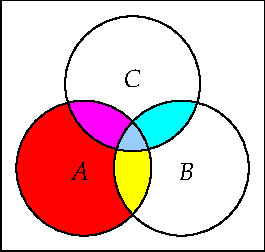
\includegraphics{sets-07-venndist}
\end{thm}


% 
% \begin{proof}
% \begin{itemize}
%   \item[($\subseteq$)] Let $x\in A\cup (B\cap C)$. Then $x\in A$ or $x\in B\cap C$. There are two cases:
%   \begin{itemize}
%     \item[(a)] If $x\in A$, then $x\in A\cup B$ and $x\in A\cup C$ by Theorem \ref{thm:setbasic}, part 2.
%     \item[(b)] If $x\in B\cap C$, then $x\in B$ and $x\in C$. It follows that $x\in A\cup B$ and $x\in A\cup C$, again by Theorem \ref{thm:setbasic}.
%   \end{itemize}
%   In both cases $x\in (A\cup B)\cap(A\cup C)$.
%   \item[($\supseteq$)] Let $y\in (A\cup B)\cap(A\cup C)$. Then $y\in A\cup B$ and $y\in A\cup C$. There are again two cases:
%   \begin{itemize}
%     \item[(a)] If $y\in A$, then we are done, for then $y\in A\cup (B\cap C)$.
%     \item[(b)] If $y\notin A$, then $y\in B$ and $y\in C$. Hence $y\in B\cap C$. In particular $y\in A\cup (B\cap C)$.
%   \end{itemize}
%   In both cases $y\in A\cup (B\cap C)$.\qedhere
% \end{itemize}
% \end{proof}


\begin{proof}
	We prove only the first result.
	\begin{align*}
		x\in A\cap(B\cup C) &\iff x\in A\text{ and }x\in B\cup C\\
		&\iff x\in A \text{ and }\bigl(x\in B\text{ or }x\in C\bigr)\\
		&\iff \bigl(x\in A \text{ and }x\in B\bigr)\text{ or }\bigl(x\in A\text{ and }x\in C\bigr) \tag{distributive law, page \pageref{pg:asidelogicalgebra}}\\
		&\iff x\in A\cap B\text{ or }x\in A\cap C\\
		&\iff x\in (A\cap B)\cup(A\cap C)\tag*{\qedhere}
	\end{align*}
\end{proof}

\goodbreak

% \paragraph{Self-test Questions}
% 
% \begin{enumerate}
%   \item The set operations of complement, union and intersection are based, respectively, on the logical constructions \underline{\phantom{not\quad}}, \underline{\phantom{or\quad}}, and \underline{\phantom{and\quad}}.
%   \item The result $\comp{(A\cup B)}=\comp A\cap\comp B$ is one of \underline{\phantom{De Morgan's laws\qquad}}.
%   \item True or false: if $A$ and $B$ are finite sets, then $A\cap B$ has strictly smaller cardinality than $A$.
%   \item True or false: if $A$ is a finite set, then $\comp A$ is a finite set.
%   \item True of false: if $A$ and $B$ are finite sets, then $\nm{A\cup B}\le\max(\nm A,\nm B)$.
% \end{enumerate}

\begin{exercises}{}{}
	A reading quiz and several questions with linked video solutions can be found \href{http://www.math.uci.edu/~ndonalds/math13/selftest/4-2-union.html}{online}.
	
	\begin{enumerate}
	  \item Describe each set simply as you can: e.g., 
	  \[
	  	\bigl\{x\in\R:x^2<9\text{ and } x^3<8\bigr\}= (-3,3)\cap(-\infty,2) =(-3,2)
	  \]
	  \begin{enumerate}
		 	\item $\bigl\{x\in\R:x^2\neq x\bigr\}$
			\item $\bigl\{x\in\R:x^3-2x^2-3x\le 0\text{ or }x^2=4\bigl\}$
			\item $\bigl\{y\in\R:\exists x\in\R \text{ with }y=x^2 \text{ and }x\neq 1\bigl\}$
			\item $\bigl\{z\in\Z:z^2\text{ is even and $z^3$ is odd}\bigl\}$
			\item $\bigl\{y\in 3\Z+2:y^2\equiv 1\spmod 3\bigl\}$
		\end{enumerate}
	  
	  \item Let $A=\{1,3,5,7,9\}$, $B=\{1,4,7,10\}$ and $\cU=\{1,2,\ldots,10\}$. What are the following sets?
	    \begin{enumerate}
		  	\item \makebox[100pt][l]{$A\cap B$\hfill (b)} \ \makebox[100pt][l]{$A\cup B$\hfill (c)} \ \makebox[100pt][l]{$B\setminus A$\hfill (d)} \ $\comp A$ 
		  	\setcounter{enumii}{4}
		  	\item \makebox[100pt][l]{$\comp{(A\setminus B)}$ \hfill (f)} \ \makebox[100pt][l]{$\comp A\cap \comp B$\hfill (g)} \ $(A\cup B)\setminus (A\cap B)$
			\end{enumerate}
	
  	
% 	\item Consider Theorems \ref{thm:setbasic} and \ref{thm:setdist}. In all seven results, replace the symbols in the first row of the following table with those in the second. Which of the results seem familar? Which are false?
% \[\begin{array}{c|c|c|c|c}
% \emptyset&A,B,C\text{ sets}&\cup&\cap&\subseteq\\\hline
% 0&A,B,C\in\N_0&+&\cdot&\le
% \end{array}\]

	%\item Prove that $B\setminus A=B\iff A\cap B=\emptyset$.
	
		\item Give formal proofs of the following parts of Theorems \ref{thm:setbasic}, \ref{thm:setcomp} and \ref{thm:setdist}. %With practice you should be able to prove \emph{all} of parts of these theorems \emph{without} looking at the arguments in the notes!
		\begin{enumerate}
		  \item \makebox[180pt][l]{$\emptyset\cap A=\emptyset$\hfill (b)} \ $A\cap (B\cap C)=(A\cap B)\cap C$
		  \setcounter{enumii}{2}
			\item \makebox[180pt][l]{$\comp{(\comp A)}=A$\hfill (d)} \ $A\cup(B\cap C)=(A\cup B)\cap(A\cup C)$
			\setcounter{enumii}{4}
			\item $A\subseteq B\iff \comp B\subseteq \comp A$
		\end{enumerate}
	
	
		\item By showing that each side is a subset of the other, give a formal proof of the set identity
		\[
			A=(A\setminus B)\cup (A\cap B)
		\]
		Now repeat your argument using only results from set algebra (Theorems \ref{thm:setcomp} and \ref{thm:setdist}).
	
	
	\item Prove the identity $A\cup B=A\iff B\subseteq A$ for any sets $A,B$.
	
	
	\item Prove the identities for any sets $A,B,C$:
	\begin{enumerate}
	  \item $\comp{(A\cap B\cap C)}=\comp A\cup\comp B\cup\comp C$
	  \item $(A\cup B)\setminus (A\cap B)=(A\setminus B)\cup (B\setminus A)$
	\end{enumerate}
	
		
	\item Prove or disprove the following conjectures (\emph{Hint: revisit Section \ref{sec:proof2}}).
	 \begin{enumerate}
	    \item $\exists x\in\R\setminus\Q$ such that $x^2\in\Q$. \qquad\qquad (b) \ $\forall x\in\R\setminus\Q$ we have $x^2\in\Q$.
		\end{enumerate}
	
	
	  \item Let $A\subseteq\R$, and let $x\in\R$. We say that $x$ is \emph{far away} from the set $A$ if and only if:
	  \[
	  	\exists d>0 \ \text{ such that } A\cap[x-d,x]=\emptyset
	  \] 
		If this does not happen, we say that $x$ is \emph{close to} $A$.
  	\begin{enumerate}
			\item Draw a picture of a set $A$ and elements $x,y$ such that $x$ is \emph{far away} from and $y$ is \emph{close to} $A$. 
			\item State the meaning of ``$x$ is close to $A$'' \ (negate ``$x$ is far away from $A$'').
			%\item Let $A=\{1,2,3\}$. Show that $x=4$ is \emph{far away} from $A$ using the definition.
			%\item Let $A=\{1,2,3\}$. Show that $x=1$ is \emph{close} to $A$.
			\item Let $A=\{1,2,3\}$.
			\begin{enumerate}
			  \item Show that $x=4$ is \emph{far away} from $A$ using the definition.
				\item Let $A=\{1,2,3\}$. Show that $x=1$ is \emph{close} to $A$.
			\end{enumerate}
			\item For general $A\subseteq\R$, show that if $x\in A$, then $x$ is \emph{close} to $A$.
			\item Let $A=(a,b)$ be a bounded interval. Is the end-point $a$ \emph{far away} from $A$?  What about $b$?
  	\end{enumerate}
  	
	\end{enumerate}

\end{exercises}

\clearpage



\subsection{Introduction to Functions}\label{sec:func1}

Sets become a lot more useful and interesting once you start transforming their elements! This is accomplished using \emph{functions.} In this section we introduce some basic concepts and notation, much of which should be familiar. A formal definition will be given in Chapter \ref{chap:relations}, but for the present the following will suffice.

\begin{defn}{}{function1}
	Let $A,B$ be sets. A \emph{function} $f:A\to B$ is a rule assigning to each input $a\in A$ a single output $b\in B$, typically denoted $f(a)$.	Various sets are associated to $f$:\par
	\begin{minipage}[t]{0.61\linewidth}\vspace{-5pt}
	\emph{Domain}: $\dom(f)=A$ is the set of inputs to the function.\smallbreak
	\emph{Codomain}: $\operatorname{codom}(f)=B$ is the set of potential outputs.\smallbreak
	\emph{Image} of a subset $U\subseteq A$: the set of outputs given inputs in $U$
	\[
		f(U):=\bigl\{f(u)\in B:u\in U\bigr\}
	\]
	\emph{Range}: $\range(f)=f(A)=\{f(a)\in B:a\in A\}$ is the set of realized outputs.
		\end{minipage}
		\hfill
		\begin{minipage}[t]{0.38\linewidth}\vspace{-3pt}
			\flushright
   		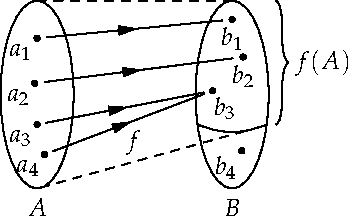
\includegraphics[scale=1]{sets-16-funcdef2}
		\end{minipage}\medbreak
	\emph{Inverse image} (or \emph{pre-image}) of a subset $V\subseteq B$: the set of inputs which are mapped into $V$
	\[
		f^{-1}(V):=\bigl\{a\in A:f(a)\in V\bigr\}
	\]
\end{defn}

The rule defining a function can be described using arrow notation $f:a\mapsto b$.

\begin{examples}{}{functions}
	\exstart Functions whose codomain is (a subset of) the real numbers $\R$ are often \textcolor{blue}{graphed}: the \textcolor{Purple}{domain} and \textcolor{Green}{range} are found by projecting the graph onto the two axes.\par
	\begin{enumerate}\setcounter{enumi}{1}
		\begin{minipage}[t]{0.6\linewidth}\vspace{-8pt}
			\item[]For instance if $f:[-3,2)\to\R$ is the square function
			\[
				f:x\mapsto x^2 \tag{equivalently $f(x)=x^2$}
			\]
			then $\textcolor{Purple}{\dom(f)=[-3,2)}$ and $\textcolor{Green}{\range(f)=[0,9]}$. We could also calculate other images/pre-images, for example,
  		\begin{gather*}
  			f\bigl([-1,2)\bigr)=\bigl\{x^2:-1\le x<2\bigr\}=[0,4)\\[3pt]
  			\begin{aligned}
  				f^{-1}\bigl((-10,2]\bigr)&=\bigl\{x\in[-3,2):-10<x^2\le 2\bigr\}\\
  				&=[-\sqrt 2,\sqrt 2]
  			\end{aligned}
  		\end{gather*}
		\end{minipage}
		\hfill
		\begin{minipage}[t]{0.39\linewidth}\vspace{-8pt}
			\flushright
  		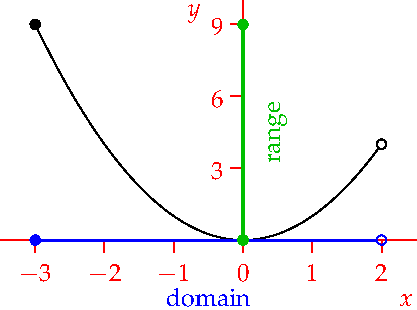
\includegraphics{sets-10-rangedom}
		\end{minipage}
		
 	  \bigbreak
		

	\begin{minipage}[t]{0.64\linewidth}\vspace{0pt}
		\item Define $f:\Z\to\{0,1,2\}$ by $f:n\mapsto n^2\pmod 3$. The table shows a few examples (remember $\dom(f)=\Z$ is infinite!).
	\end{minipage}
	\hfill
	\begin{minipage}[t]{0.35\linewidth}\vspace{0pt}
		\flushright
		$\begin{array}{c|cccccccc}
  		n&0&1&2&3&4&5&6&7\\\hline
  		f(n)&0&1&1&0&1&1&0&1
  	\end{array}$
	\end{minipage}\par
		Exercise \ref*{sec:cong}.\ref{exs:nsquaredrem} confirms what the examples suggest, that $\range(f)=\{0,1\}$. We also compute a single inverse image (revisit the previous two sections if you're unsure about the notation):
		\begin{align*}
			f^{-1}\bigl(\{1\}\bigr) &=\bigl\{x\in\Z:x^2\equiv 1\spmod 3\bigr\} =\bigl\{x\in\Z:x\equiv 1\text{ or }2\spmod 3\bigr\}\\
			&=(3\Z+1)\cup(3\Z+2)
		\end{align*}

  \begin{minipage}[t]{0.64\linewidth}\vspace{0pt}
    \item\label{ex:functmod} Let $A=\{0,1,2,\ldots,7\}$ be the set of remainders modulo 8 and define two functions $f,g:A\to A$:
    \[
    	f(n)=3n\spmod{8}\qquad g(n)=6n\spmod 8
    \]
  \end{minipage}
  \hfill
  \begin{minipage}[t]{0.35\linewidth}\vspace{0pt}
  	\flushright
  	$\begin{array}{c|cccccccccc}
  		n&0&1&2&3&4&5&6&7\\\hline
  		f(n)&0&3&6&1&4&7&2&5\\\hline
  		g(n)&0&6&4&2&0&6&4&2
  	\end{array}$	
  \end{minipage}
  \smallbreak
  Since the domain has only 8 elements, the table describes everything. Observe that
  \begin{align*}
  	&\range(f)=A &&f\bigl(\{1,5\}\bigr) =\{3,7\} &&f^{-1}\bigl(\{1,2,3,4\}\bigr) =\{1,3,4,6\}\\
  	&\range(g)=\{0,2,4,6\} &&g\bigl(\{1,5\}\bigr) =\{6\} &&g^{-1}\bigl(\{1,2,3,4\}\bigr) =\{2,3,6,7\}
  \end{align*}
  	
  \item Let $A=\{0,1,2,3,4\}$ and let $B=\{$two-element subsets of $A\}$. Define
  \[
  	f:A\to B:a\mapsto \{a,a+1\negthickspace \spmod 5\}
  \]
  where we take the remainder modulo 5. You should be able to convince yourself that
  \begin{gather*}
  	\range(f)=\big\{ \{0,1\}, \{1,2\}, \{2,3\}, \{3,4\}, \{4,0\} \big\}\\[3pt]
  	f\bigl(\{1,4\}\bigr)=\big\{f(1),f(4)\big\}=\big\{\{1,2\},\{4,0\}\big\} \quad\text{and}\quad f^{-1}\bigl\{\{2,4\},\{4,0\}\bigr\}=\{4\}
  \end{gather*}
	\end{enumerate}
  
\end{examples}


\boldsubsubsection{Injections, Surjections and Invertibility}

We turn our attention to perhaps the most important properties a function can possess.

\begin{defn}{}{11}
	Let $f:A\to B$ be a function. We say that $f$ is:
	\begin{enumerate}
	  \item \emph{Injective} (\emph{1--1}, an \emph{injection}) if it never outputs the same value twice. Equivalently,\footnotemark{}
		\[
			f(a_1)=f(a_2)\implies a_1=a_2 \tag{``$\forall a_1,a_2\in A$'' is typically hidden}
		\]
		\item \emph{Surjective} (\emph{onto}, a \emph{surjection}) if every possible output is realized: $B=\range(f)$. Equivalently,${}^{\thefootnote}$
		\[
			\forall b\in B,\ \exists a\in A\text{ such that }f(a)=b
		\]
		\item \emph{Bijective} (\emph{invertible}, a \emph{bijection}) if it is both injective and surjective. Equivalently
		\[
			\forall b\in B,\ \exists \text{ a \emph{unique} }a\in A\text{ such that }f(a)=b
		\]
		When $f$ is bijective, its \emph{inverse function} is $f^{-1}:B\to A:b\mapsto a$.
	\end{enumerate}
\end{defn}

\footnotetext{For injectivity this is the contrapositive: if $f$ never takes the same value twice, then $a_1\neq a_2\implies f(a_1)\neq f(a_2)$.\par
For surjectivity, the quantified statement expresses $B\subseteq\range(f)$. The inclusion $\range(f)\subseteq B$ is true for \emph{any} function.}


Since the definitions of injectivity and surjectivity are both universal statements, it suffices to provide \emph{counter-examples} to show that a function is \emph{not injective} or \emph{not surjective.} Indeed:
\[
	\tcbhighmath{
		\begin{array}{@{}ll}
			\text{\emph{$f$ not injective}:}&\text{$\exists a_1\neq a_2\in A$ such that $f(a_1)=f(a_2)$}\\[5pt]
			\text{\emph{$f$ not surjective}:}&\text{$\exists b\in B$ such that $\forall a\in A$, $f(a)\neq b$}
		\end{array}
	}
\]

\goodbreak

\begin{examples*}{\ref{ex:functions}, cont.}{}
	We briefly revisit our previous examples.
	\begin{enumerate}
	  \item Let $f:[-3,2)\to\R:x\mapsto x^2$.
	  \begin{itemize}
	  	\item $f$ is non-injective: $f(1)=f(-1)$ provides a counter-example. \hfill ($a_1=1=-a_2$)
	  	\item $f$ is non-surjective: there is no $x\in[-3,2)$ for which $x^2=-5$. \hfill ($b=-5$)
	  \end{itemize}
	  
	  
	  \begin{minipage}[t]{0.73\linewidth}\vspace{-3pt}
	  	We can obtain a related injective function by shrinking the domain, for instance $g:\textcolor{Purple}{[0,2)}\to\R:x\mapsto x^2$.	Indeed
	  	\[
	  		g(x_1)=g(x_2) \implies x_1^2=x_2^2 \implies x_1=x_2
	  	\]
	  	since $x_1,x_2\in\textcolor{Purple}{[0,2)}$ are non-negative. By also shrinking the codomain, we get a surjective (now \emph{bijective}) function: $h:\textcolor{Purple}{[0,2)}\to \textcolor{Green}{[0,4)}:x\mapsto x^2$.
	  	\medbreak
	  	\emph{Proof of surjectivity}: Given $\textcolor{Green}{y\in[0,4)}$, let $\textcolor{Purple}{x}=\sqrt{\textcolor{Green}{y}}$, then $y=h(x)$.
	  \end{minipage}
	  \hfill
	  \begin{minipage}[t]{0.26\linewidth}\vspace{-3pt}
	  	\flushright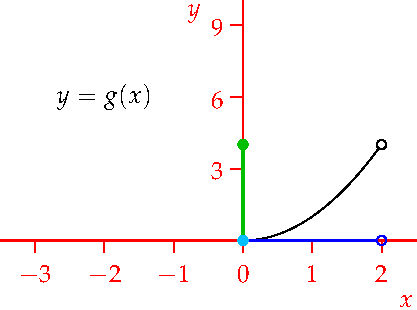
\includegraphics{sets-18-rangedom2}
	  \end{minipage}

% 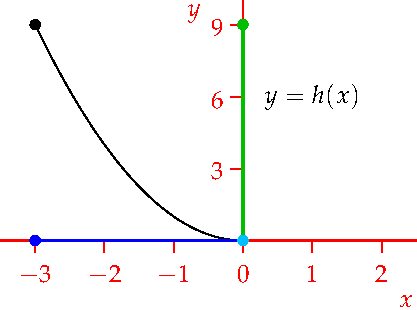
\includegraphics[width=0.4\textwidth]{sets-19-rangedom3}


% 	  \begin{minipage}[t]{0.7\linewidth}\vspace{0pt}
% 	  	\item $f$ is neither injective ($f(a_3)=f(a_4)$) nor surjective $b_4\notin\range(f)$.
% 	  \end{minipage}
% 	  \hfill
% 	  \begin{minipage}[t]{0.29\linewidth}\vspace{0pt}
% 	  	\flushright
% 	  	$\begin{array}{c|cccc}
%   		a&a_1&a_2&a_3&a_4\\\hline
%   		f(a)&b_1&b_2&b_3&b_3
%   		\end{array}$
% 	  \end{minipage}


  	\item $f:\Z\to\{0,1,2\}:n\mapsto n^2\spmod 3$ is neither injective nor surjective.
  	\begin{itemize}
  		\item $f$ is non-injective: for instance $f(1)=f(2)$.
  		\item $f$ is non-surjective: $\range(f)=\{0,1\}\neq \{0,1,2\}=\operatorname{codom}(f)$.
		\end{itemize}
	
		\begin{minipage}[t]{0.64\linewidth}\vspace{-10pt}
    	\item Given $f,g:A\to A$ where $A=\{0,1,\ldots,7\}$ as in the table:
    	\begin{itemize}\itemsep0pt
      	\item $f$ is bijective: all elements of $\operatorname{codom}(f)$ appear exactly once in the $f$-row.
     	 	\item $g$ is non-injective: e.g., $g(0)=g(4)$.
      	\item $g$ is non-surjective: e.g., $1\notin\range(g)=\{0,2,4,6\}$.
    	\end{itemize}
  	\end{minipage}
  	\hfill
  	\begin{minipage}[t]{0.35\linewidth}\vspace{-10pt}
  		\flushright
  		$\begin{array}{c|cccccccccc}
  			n&0&1&2&3&4&5&6&7\\\hline
  			f(n)&0&3&6&1&4&7&2&5\\\hline
  			g(n)&0&6&4&2&0&6&4&2
  		\end{array}$	
  	\end{minipage}

  
	  \item Let $A=\{0,1,2,3,4\}$ and $f:A\to\bigl\{$two-element subsets of $A\bigr\}:a\mapsto \{a,a+1\spmod 5\}$
	  \begin{itemize}%\itemsep0pt
	    \item $f$ is injective: suppose $a_1,a_2\in A$, then
	    \[
	  		f(a_1)=f(a_2)\implies \{a_1,a_1+1\negthickspace\spmod 5\}=\{a_2,a_2+1\negthickspace\spmod 5\}\implies a_1=a_2
	  	\]
	  	\item $f$ is not surjective: e.g., $\{1,3\}\notin\range(f)$.
	  \end{itemize}
    
	\end{enumerate}
\end{examples*}


%To show that a function is bijective, it is enough to exhibit an inverse function. 
You should have seen the approach of the next example in other classes.

\begin{example}[lower separated=false, sidebyside, sidebyside align=top seam, sidebyside gap=0pt, righthand width=0.28\linewidth]{}{}
	We show that $f:(-\infty,2)\to (1,\infty): x\mapsto 1+\frac 1{(x-2)^2}$ is bijective by \emph{computing its inverse function.} Just solve for $x$ in terms of $y$: 
	\begin{align*}
		y=1+\frac 1{(x-2)^2}&\implies (x-2)^2=\frac 1{y-1}\\
		&\implies f^{-1}(y)=x=2-\frac 1{\sqrt{y-1}}
	\end{align*}
	The sign of the square-root was chosen so that $x\in\dom(f)=(-\infty,2)$.
	\tcblower
  \flushright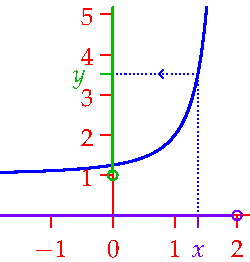
\includegraphics{sets-09-bij2}
\end{example}

\goodbreak

% 
% \begin{aside}{}{}
% {\bf Inverse Functions}
% 
% The word \emph{invertible} is a synonym for bijective because bijective functions really have inverses! Indeed, suppose that $f:A\to B$ is bijective. Since $f$ is surjective, we know that $B=\range(f)$ and so every element of $B$ has the form $f(a)$ for some $a\in A$. Moreover, since $f$ is injective, the $a$ in question is unique. The upshot is that, when $f$ is bijective, we can construct a new \emph{function}
% \[f^{-1}:B\to A:f(a)\mapsto a.\]
% This may appear difficult at the moment but we will return to it in Chapter \ref{chap:relations}.
% 
% Instead, recall that in Calculus you saw that any injective function has an inverse. How does this fit with our definition? Consider, for example, $f:[0,2]\to\R:x\mapsto x^4$. This is injective but not surjective. To fix this, simply define a new function with the same formula but with codomain equal to the range of $f$. We obtain the bijective function
% \[g:[0,2]\to[0,16]:x\mapsto x^4,\]
% with inverse
% \[g^{-1}:[0,16]\to[0,2]:x\mapsto \sqrt[4]{x}.\]
% In Calculus we didn't nitpick like this and would simply go straight to $f^{-1}(x)=\sqrt[4]{x}$.\\[5pt]
% In general, if $f:A\to B$ is any injective function, then $g:A\to f(A):x\mapsto f(x)$ is automatically bijective, since we are forcing the codomain of $g$ to match its range.
% \end{aside}



\boldsubsubsection{Composition of Functions}

We consider how injectivity and surjectivity interact with composition of functions.

\begin{defn}[lower separated=false, sidebyside, sidebyside align=top seam, sidebyside gap=0pt, righthand width=0.4\linewidth]{}{}
	Given functions $f:A\to B$ and $g:B\to C$, their \emph{composition} is the function
	\[
		\textcolor{red}{g\circ f}:A\to C:a\mapsto g\bigl(f(a)\bigr)
	\]
	Note the order: to compute $(g\circ f)(a)$, first apply $f$, then $g$.
	\tcblower
	\flushright
	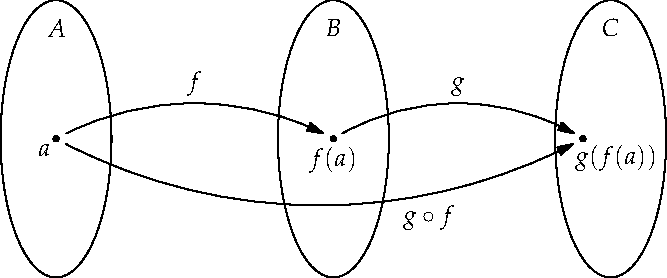
\includegraphics[scale=1]{sets-15-setcomp}
\end{defn}

In practice, some restriction of domains might be required in order to define a composition.

\begin{example}{}{}
	If $f(x)=x^2$ and $g(x)=\frac 1{x-1}$, then
	\[
		(g\circ f)(x)=\frac 1{x^2-1}\quad\text{and}\quad(f\circ g)(x)=\frac 1{(x-1)^2}
	\]
	Even though $\pm 1$ are legitimate inputs for $f$, $\dom(g\circ f) =\R\setminus\{\pm 1\}$ is implied so as to prevent division by zero. 
\end{example}


\begin{thm}{}{compinjsurj}
	Let $f:A\to B$ and $g:B\to C$ be functions. Then:
	\begin{enumerate}
	  \item If $f$ and $g$ are injective, then $g\circ f$ is injective.
	  \item If $f$ and $g$ are surjective, then $g\circ f$ is surjective.
	\end{enumerate}
	It follows that the composition of bijective functions is also bijective.
\end{thm}

\begin{proof}
	Suppose $f$ and $g$ are injective and let $a_1,a_2\in A$. Then
  \begin{align*}
  (g\circ f)(a_1)=(g\circ f)(a_2)&\implies g\big(f(a_1)\big)=g\big(f(a_2)\big)\\
  &\implies f(a_1)=f(a_2)\tag*{(since $g$ is injective)}\\
  &\implies a_1=a_2\tag*{(since $f$ is injective)}\\[-25pt]
  \end{align*}
%   \item Now suppose that $f$ and $g$ are surjective. Let $c\in C$. We are required to show that $\exists a\in A$ such that $(g\circ f)(a)=c$.\\
%   Since $g$ is surjective, $\exists b\in B$ such that $g(b)=c$.\\
%   Similarly, since $f$ is surjective, $\exists a\in A$ such that $f(a)=b$.\\
%   Together we have $(g\circ f)(a)=g(f(a))=c$, as required.
%\end{enumerate}
	That is, $g\circ f$ is injective. We leave part 2 to the exercises.
\end{proof}

Somewhat surprisingly, the converse of this theorem is \emph{false.} If a composition is injective or surjective, \emph{only one} of the original functions is required also to be.

\begin{thm}[lower separated=false, sidebyside, sidebyside align=top seam, sidebyside gap=0pt, righthand width=0.4\linewidth]{}{}
Suppose $f:A\to B$ and $g:B\to C$.
\begin{enumerate}
  \item If $g\circ f$ is injective, then $f$ is injective.
  \item If $g\circ f$ is surjective, then $g$ is surjective.
\end{enumerate}
The picture illustrates what can happen: $f$ is \emph{only injective}, $g$ is \emph{only surjective,} but $g\circ f$ is \emph{bijective.}
	\tcblower
	\flushright
	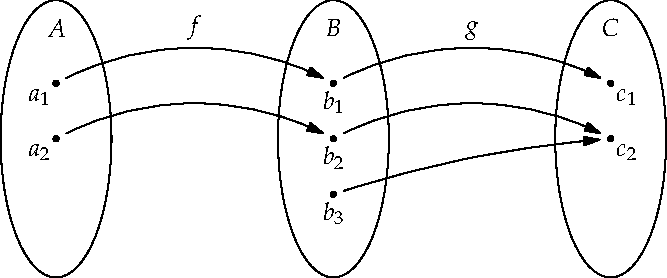
\includegraphics[scale=1]{sets-17-injcomp}
\end{thm}


\goodbreak

\begin{example}{}{}
	Here is a formulaic version of the picture in the theorem. Make sure you're comfortable with the definitions and draw pictures or graphs to help make sense of what's going on.
	\begin{gather*}
		f:[0,2]\to[-4,4]:x\mapsto x^2\tag{injective only}\\
		g:[-4,4]\to [0,16]:x\mapsto x^2\tag{surjective only}\\
		g\circ f:[0,2]\to[0,16]:x\mapsto x^4\tag{bijective!}
	\end{gather*}
\end{example}


\begin{proof}
% \begin{enumerate}\setcounter{enumi}{1}
%   \item Suppose that $f(a_1)=f(a_2)$. Then $(g\circ f)(a_1)=(g\circ f)(a_2)$. Since $g\circ f$ is injective we conclude that $a_1=a_2$, whence $f$ is injective.\qedhere
	This time we leave part 1 for the Exercises. Let $c\in C$ and assume $g\circ f$ is surjective. But then
	\begin{align*}
		&\exists a\in A\text{ such that } c=(g\circ f)(a)=g\bigl(f(a)\bigr)
	\end{align*}
	Otherwise said, $\exists b(=f(a))\in B$ for which $c=g(b)$: that is, $g$ is surjective.%\qedhere
% \end{enumerate}
\end{proof}


\boldsubsubsection{Functions and Cardinality}

Injectivity and surjectivity are intimately tied to the notion of cardinality. In Chapter \ref{chap:cantor}, we will use such functions to \emph{define} cardinality for infinite sets. For the present we stick to finite sets. 

\begin{thm}{}{finitecard}
	Let $A$ and $B$ be finite sets. The following are equivalent:
	\begin{enumerate}\itemsep0pt
	  \item $\nm A\le\nm B$ \qquad\qquad 2. \ $\exists f:A\to B$ injective \qquad\qquad 3. \ $\exists g:B\to A$ surjective
	\end{enumerate}
	Moreover, $\nm A=\nm B\iff\exists f:A\to B$ bijective.
\end{thm}

\begin{minipage}[t]{0.84\linewidth}\vspace{-3pt}
	The theorem asserts that \emph{any one} of the three numbered statements is true if and only if \emph{all} are. It might appear that six arguments are required but, by proving in a circle, we only need three: for instance \circint 1 $\Rightarrow$ \circint 3 holds because \circint 1 $\Rightarrow$ \circint 2 and \circint 2 $\Rightarrow$ \circint 3.\par
	The proof is very abstract, but if you focus on the picture it should make sense.
\end{minipage}
\hfill
\begin{minipage}[t]{0.15\linewidth}\vspace{-3pt}
	\flushright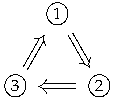
\includegraphics{sets-14-circlearg}%\vspace{-10pt}
\end{minipage}
\par


\begin{proof}
Suppose $\nm A=m$, $\nm B=n$ and label the elements in roster notation:\par
\begin{minipage}[t]{0.63\linewidth}\vspace{-14pt}
\[
	A=\{a_1,a_2,\ldots,a_m\}\qquad B=\{b_1,b_2,\ldots,b_n\}
\]
\begin{description}
	\item[\normalfont \circint 1 $\Rightarrow$ \circint 2]
	If $m\le n$, \emph{define} $f:A\to B$ by $f(a_k)=b_k$ as in the picture. This is injective since the $b_1,\ldots,b_m$ are distinct.
\end{description}
\end{minipage}
\hfill
\begin{minipage}[t]{0.3\linewidth}\vspace{-20pt}
	\flushright
	$\xymatrix @C0pt @R10pt @M1.4pt @H15pt{
		\{a_1, \ar@{|->}[d]_f &a_2,&\ldots,&a_m\} \ar@<-1ex>@{|->}[d]_f\\
		\{b_1, \ar@<-1ex>@{|->}[u]_g &b_2,&\ldots,&b_m, \ar@<0ex>@{|->}[u]_g&\overbrace{b_{m+1},\ldots,b_n}\} \ar@(u,ur)@{|->}@/_3pc/[ullll]_g
	}$
\end{minipage}
\vspace{-2pt}
\begin{description}%\itemsep0pt
	\item[\normalfont \circint 2 $\Rightarrow$ \circint 3] Suppose $f:A\to B$ is injective. Without loss of generality, label the elements of $B$ such that $b_k=f(a_k)$ for $1\le k\le m$. \emph{Define} the surjective function $g:B\to A$ as in the picture:\footnotemark{}%\vspace{-2pt}
  \[
  	g(b_k):=
  	\begin{cases}
  		a_k&\text{ if }k\le m\\
  		a_1&\text{ if }k>m
  	\end{cases}
  \]
  \item[\normalfont \circint 3 $\Rightarrow$ \circint 1] Suppose $g:B\to A$ is surjective. Without loss of generality, label the elements of $B$ such that $a_k=g(b_k)$ for $1\le k\le m$. Since the $b_k$ must be distinct, we see that $n\ge m$.
\end{description}
When $m=n$, the constructed functions are plainly \emph{bijections} with $f^{-1}=g$.
\end{proof}

\vspace{-5pt}

\footnotetext{The elements $b_{m+1},\ldots,b_n$ could be mapped \emph{anywhere,} we choose $a_1$ for simplicity.}

\goodbreak



\begin{exercises}
	A reading quiz and several questions with linked video solutions can be found \href{http://www.math.uci.edu/~ndonalds/math13/selftest/4-3-functions.html}{online}.

	\begin{enumerate}
	  \item For each of the following functions $f:A\to B$ determine whether $f$ is injective, surjective or bijective. Prove your assertions.
	  \begin{enumerate}
	    \item $f:[0,3]\to\R$ where $f(x)=2x$.
	    \item $f:[3,12)\to[0,3)$ where $f(x)=\sqrt{x-3}$.
	    \item $f:(-4,1]\to(-5,-3]$ where $f(x)=-\sqrt{x^2+9}$.
	  \end{enumerate}
	  
	  
	  \item Suppose that $f:[-3,\infty)\to[-8,\infty)$ and $g:\R\to\R$ are defined by
		\[
			f(x)=x^2+6x+1,\qquad\qquad g(x)=2x+3
		\]
		Compute $g\circ f$ and show that it is injective.
	  
	  
	  \item\begin{enumerate}
			\item Find a set $A$ so that the function $f:A\to\R:x\mapsto\sin x$ is injective.
			\item Find a set $B$ so that the function $f:\R\to B:x\mapsto\sin x$ is surjective.
		\end{enumerate}
	

	  \item A function $f:\R\to\R$ is \emph{even} if and only if $\forall x\in\R,\ f(-x)=f(x)$.
		\begin{enumerate}
			\item Prove that $f:x\mapsto x^2$ is even.
			\item By negating the definition, state what it means for a function \emph{not to be even.}
			\item Give an example of a function that is \emph{not} even: prove it. 
			\item Prove or disprove: for every $f,\,g:\R\to\R$ even, the composition $h=f\circ g$ is even.
		\end{enumerate}
		
		
		\begin{minipage}[t]{0.6\linewidth}\vspace{0pt}
			\item The picture in Definition \ref{defn:function1} illustrates a function
			\[
				f:\{a_1,a_2,a_3,a_4\}\to\{b_1,b_2,b_3,b_4\}
			\]
			State the following:\vspace{-2pt}
		\end{minipage}
		\hfill
		\begin{minipage}[t]{0.39\linewidth}\vspace{0pt}
			\flushright
			$\begin{array}{c|cccc}
	   		a&a_1&a_2&a_3&a_4\\\hline
	   		f(a)&b_1&b_2&b_3&b_3
	  	\end{array}$
		\end{minipage}	
		\begin{enumerate}
		  \item $\range(f)$\qquad\qquad (b) \ $f\bigl(\{a_1,a_4\}\bigr)$\qquad\qquad (c) \ $f^{-1}\bigl(\{b_3\}\bigr)$\qquad\qquad (d) \ $f^{-1}\bigl(\{b_4\}\bigr)$
		\end{enumerate}
	
	
		\item\begin{enumerate}
	    \item Let $A=\{a,b,c\}$, $B=\{1,2,3,4\}$ and $f:A\to B$ be the function defined by $f(a)=f(c)=1$ and $f(b)=3$. State the following:
	    	\begin{enumerate}
	    	  \item $f^{-1}\bigl(\{1\}\bigr)$\qquad\qquad (b) \ $f^{-1}\bigl(\{3\}\bigr)$\qquad\qquad (c) \ $f^{-1}\bigl(\{1,3\}\bigr)$\qquad\qquad (d) \ $f^{-1}\bigl(\{2,4\}\bigr)$
	    	\end{enumerate} 
	    \item Let $g:[-1,\infty)\to\R:x\mapsto x^2+2x+1$. Compute $g^{-1}\bigl((0,2]\bigr)$. 
	    \item Let $h:\R\to\R:x\mapsto \sin x$. Find $h^{-1}\bigl(\{-1,1\}\bigr)$. 
		\end{enumerate}
	
		
	  \item Define $f:(-\infty,0]\to\R$ and $g:[0,\infty)\to\R$ by
	  \[
	  	f(x)=x^2,\qquad g(x)=
	  	\begin{cases}
	  		\frac{x}{1-x}&x<1\\
	  		1-x&x\ge 1
	  	\end{cases}
	  \]
	  Is $g\circ f:(-\infty,0]\to\R$ surjective? Justify your answer.
		  
	  
	  \item\label{ex:kfunc} Recall Example \ref*{ex:functions}.\ref{ex:functmod}.
	  Consider the nine functions $f_k:A\to A:x\mapsto kx\pmod{10}$, where $k=1,2,\ldots,9$. Find the range of each $f_k$. Can you find a relationship between $k$ and the cardinality of $\range(f_k)$?
			%\item More generally, let $A=\{0,1,2\ldots,n-1\}$ be the set of remainders modulo $n$. If $f_k:A\to A:x\mapsto kx\spmod n$, conjecture a relationship between $\nm{\range(f_k)}$, $k$ and $n$. You don't need to prove your assertions.
	  
	  
	 	\goodbreak
	 
	  
	  \item Let $f:\R\to\R^+$ be the function defined by $f(x)=e^x$. Explain why the following ``proof'' that $f$ is surjective is incorrect. Then, give a correct proof.  
		\begin{proof}[Proof?]
			Let $e^x\in\R^+$ be arbitrary. Then $f(x)=e^x$. We conclude that $f$ is surjective.
		\end{proof}
		
	
		\item\begin{enumerate}
		  \item Show there is a bijection between $\Z$ and $2\Z$.
			\item Let $S$ be the set of all circles in the plane which are centered at the origin. Find a bijection between $S$ and $\R^+$.
			\item Let $A,B$ be \emph{finite} sets. If $A\subsetneq B$, is it possible for there to be a bijection between $A$ and $B$?
		\end{enumerate}
	
	
	  \item Prove that the composition of two surjective functions is surjective.
	  
	  
	  \item Suppose that $g\circ f$ is injective. Prove that $f$ is injective.
	  
	
	  \item Let $f:A\to B$. Prove the following:
	  \begin{enumerate}
	    \item $f$ is injective if and only if $\forall b\in B,\ f^{-1}\bigl(\{b\}\bigr)$ has \emph{at most} one element.
	    \item $f$ is surjective if and only if $\forall b\in B,\ f^{-1}\bigl(\{b\}\bigr)$ has \emph{at least} one element.
	  \end{enumerate}
	  
	  
		\item Prove that functional composition is associative. That is, if $f:A\to B$, $g:B\to C$, and $h:C\to D$ are functions, then for all $a\in A$ we have
			\[
				\bigl(f\circ(g\circ h)\bigr)(a) = \bigl((f\circ g)\circ h\bigr)(a)
			\]
	  
	  \item Following Theorem \ref{thm:compinjsurj}, the composition of bijective functions $f,g$ is itself bijective. Give a \emph{brief} explanation as to why $(g\circ f)^{-1}=f^{-1}\circ g^{-1}$.
	
		
		\item Let $f:A\to B$ and $X\subseteq A$. Fill in the blanks to complete a proof of the following facts:
		\begin{enumerate}
	  	\item $X\subseteq f^{-1}\bigl(f(X)\bigr)$.\qquad\qquad\qquad (b) \ If $f$ is injective, then $X=f^{-1}\bigl(f(X)\bigr)$.
		\end{enumerate}
		\begin{proof}
			\begin{enumerate}
		  	\item $x\in X\Longrightarrow f(x)\in \underline{\phantom{f(X)}}$. Let $y=f(x)$, then $x\in \underline{\phantom{f^{-1}\bigl(\{y\}\bigr)}} \subseteq f^{-1}\bigl(f(X)\bigr)$.
		  	\item $a\in f^{-1}\bigl(f(X)\bigr) \Longrightarrow \underline{\phantom{f(a)\in f(X)}}$, whence $\exists x\in X$ with $f(a)=f(x)$. By injectivity, \underline{\phantom{$x=a$}}, whence $a\in X$. We conclude that \underline{\phantom{$f^{-1}\bigl(f(X)\bigr)\subseteq X$}}. Combine with part (a) for the result.\qedhere
			\end{enumerate}
		\end{proof}
		
	
		\item Let $f:A\to B$ be a function and let $Y\subseteq B$. Prove the following facts:
		\begin{enumerate}
	    \item $f\bigl(f^{-1}(Y)\bigr) \subseteq Y$.\qquad\qquad\qquad (b) \ If $f$ is surjective, then $f\bigl(f^{-1}(Y)\bigr)=Y$.
		\end{enumerate}
	  
	
	
		\item (Hard)\lstsp Let $f:A\to B$ be a function and $X,Y\subseteq A$.
		\begin{enumerate}
		  \item Prove that $f(X\cap Y)\subseteq f(X)\cap f(Y)$.
		  \item If $f$ is injective, prove that $f(X\cap Y) = f(X) \cap f(Y)$.
		  \item If $f(X\cap Y)=f(X)\cap f(Y)$ for \emph{all} $X,Y\subseteq A$, prove that $f$ is injective.
		\end{enumerate}
		
		
		
	
	%   \item (\emph{If you did Exercise \ref*{sec:quant}.\ref{ex:decreasing} you should find this easy}) Let $X$ be a subset of $\R$. A function $f:X\to\R$ is \emph{strictly increasing} if 
	% 	\[\forall \,a,\, b \in X,\quad a<b \Longrightarrow f(a)<f(b).\]
	% 	For example, the function $f \colon [0,\,\infty)\to \R, \,x \mapsto x^2$  is increasing because 
	% 	\[\forall a,\,b \in  [0,\,\infty) , \quad a<b \Longrightarrow f(a) = a^2< b^2=f(b).\]
	% 		\begin{enumerate}
	% 	  	\item Give another example of a function that is increasing. Draw its graph, and prove that  the function is increasing.  
	% 	  	\item By negating the above definition, state what it means for a function \emph{not to be strictly increasing.} 
	% 	  	\item Give an example of a function that is \emph{not} strictly increasing. Draw its graph, and prove that the function is not strictly increasing.  
	% 	  	\item Let $f,\,g:\R\to\R$ be strictly increasing. Prove or disprove: The function $h=f+g$ is strictly increasing. Note that the formula for $h$ is $h(x)=f(x)+g(x)$.
	% 		\end{enumerate}	
			
	%   \item You may assume that $g:[2,\infty)\to\R:x\mapsto \sqrt{x^3-8}$ is an injective function. Find a function $f:\R\to\R$ which is \emph{not injective,} but for which the composition $f\circ g:[2,\infty)\to\R$ \emph{is injective.} Justify your answer.
	
	% \item Let $f : A \to B$ be a function. Let $X_1,X_2 \subseteq A$. Prove or disprove the following:
	% \begin{enumerate}
	%     \item $X_1 \subseteq X_2$ implies $f(X_1) \subseteq f(X_2)$.
	%     \item $f(X_1 \cup X_2) = f(X_1) \cup f(X_2)$.
	%     \item $f(X_1 \cap X_2) \subseteq f(X_1) \cap f(X_2)$. 
	%     \item $f(X_1) \cap f(X_2) \subseteq f(X_1 \cap X_2)$.
	%     %\item If $f$ is injective, then $f(X_1 \cap X_2) = f(X_1) \cap f(X_2)$.
	%     %\item $f(X_1) \setminus f(X_2) \subseteq f(X_1 \setminus X_2)$.
	% \end{enumerate}
	
% \item Let $f : A \to B$ be a function and $Y_1,Y_2 \subseteq B$.
% \begin{enumerate}
% \item Prove $f^{-1}(Y_1 \cup Y_2) = f^{-1}(Y_1) \cup f^{-1}(Y_2)$.
% \item Prove $f^{-1}(Y_1 \cap Y_2) = f^{-1}(Y_1) \cap f^{-1}(Y_2)$.
% \end{enumerate}



% \item (Uses calculus) This exercise will give an example of how to use calculus to prove some properties of (certain) functions. Let $f : (-\pi/2,\pi/2) \to \R$ be defined by $f(x) = \tan x$. Recall that $f$ is differentiable, and hence continuous, on its domain.
% \begin{enumerate}
%     \item Compute $\lim_{x \to \frac{\pi}{2}^-} f(x)$ and $\lim_{x \to \frac{-\pi}{2}^+} f(x)$.
%     \item Recall the Intermediate Value Theorem: if $g : [a,b] \to \R$ is a continuous function, then for any $y$ between $g(a)$ and $g(b)$, there is $x \in [a,b]$ such that $g(x) = y$. Use the Intermediate Value Theorem and the results of part 1 to prove $f$ is surjective.
%     \item Why is a strictly increasing function (see Exercise 4.4.4) injective? 
%     \item Compute $\frac{d}{dx}f(x)$ and use this to show $f$ is strictly increasing, and therefore injective by part 3.
% \end{enumerate}
	\end{enumerate}

\end{exercises}

